\documentclass[10pt,twocolumn]{article}
\usepackage[margin=0.75in]{geometry}
\usepackage{graphicx}
\usepackage{booktabs}
\usepackage{amsmath}
\usepackage{hyperref}
\usepackage{times}
\usepackage{microtype}
\usepackage{caption}
\usepackage{subcaption}
\usepackage{xurl}

\title{SyntheticShield: Auditing Memorization and Membership Leakage in Synthetic Data Generators}
\author{Tejas Mahajan\\Department of Computer Science\\University of Central Florida}
\date{}

\begin{document}
\maketitle

\begin{abstract}
Synthetic data is often treated as a privacy-preserving replacement for sensitive datasets. However, synthetic generators can memorize rare records, duplicate outliers, or reproduce training examples with small perturbations. This paper presents \textsc{SyntheticShield}, a lightweight audit framework for measuring privacy leakage in tabular synthetic data. The framework inserts rare canary records into a private dataset, trains synthetic generators under multiple defense settings, and evaluates leakage using nearest-neighbor exposure, membership inference, and canary recovery metrics. In a controlled benchmark, a memorization-prone no-defense generator achieves high downstream utility but also produces the largest membership leakage and canary exposure. DP-inspired training and deduplication reduce exposure, demonstrating that simple privacy audits can reveal generator-specific leakage before synthetic data is released.
\end{abstract}

\section{Introduction}
Synthetic data is increasingly used to share, test, and analyze data without releasing the original private records. The core promise is appealing: a generator learns population-level structure and emits artificial samples that preserve utility while hiding individual training examples. In practice, this promise can fail when the generator memorizes rare training records or reproduces outliers. These failures are especially concerning for tabular domains, where unusual combinations of demographic, financial, or behavioral attributes can uniquely identify individuals.

This paper introduces \textsc{SyntheticShield}, an audit pipeline for measuring memorization and membership leakage in synthetic data generators. The audit treats synthetic data release as an attack surface: if a generated sample is unusually close to a private training row, then an adversary may infer that the row was used during training. We operationalize this idea using nearest-neighbor distances, membership inference, and inserted canary records whose rarity is controlled by the experiment.

\section{Threat Model}
We consider an adversary who receives a released synthetic dataset and has candidate records that may or may not have appeared in the private training set. The adversary computes how close each candidate is to the synthetic release. A candidate that has a very small nearest-neighbor distance to the synthetic data is predicted as a member. This threat model captures practical data-release settings in which an attacker may know partial records from public sources, data brokers, or previous breaches.

\section{SyntheticShield Method}
Figure~\ref{fig:main} summarizes the pipeline. First, the benchmark creates a private training set and injects canary records. Second, a synthetic generator is trained under a selected defense. Third, the generated samples are audited with distance-based privacy tests. Finally, the framework reports utility and leakage metrics side by side.

\begin{figure*}[t]
    \centering
    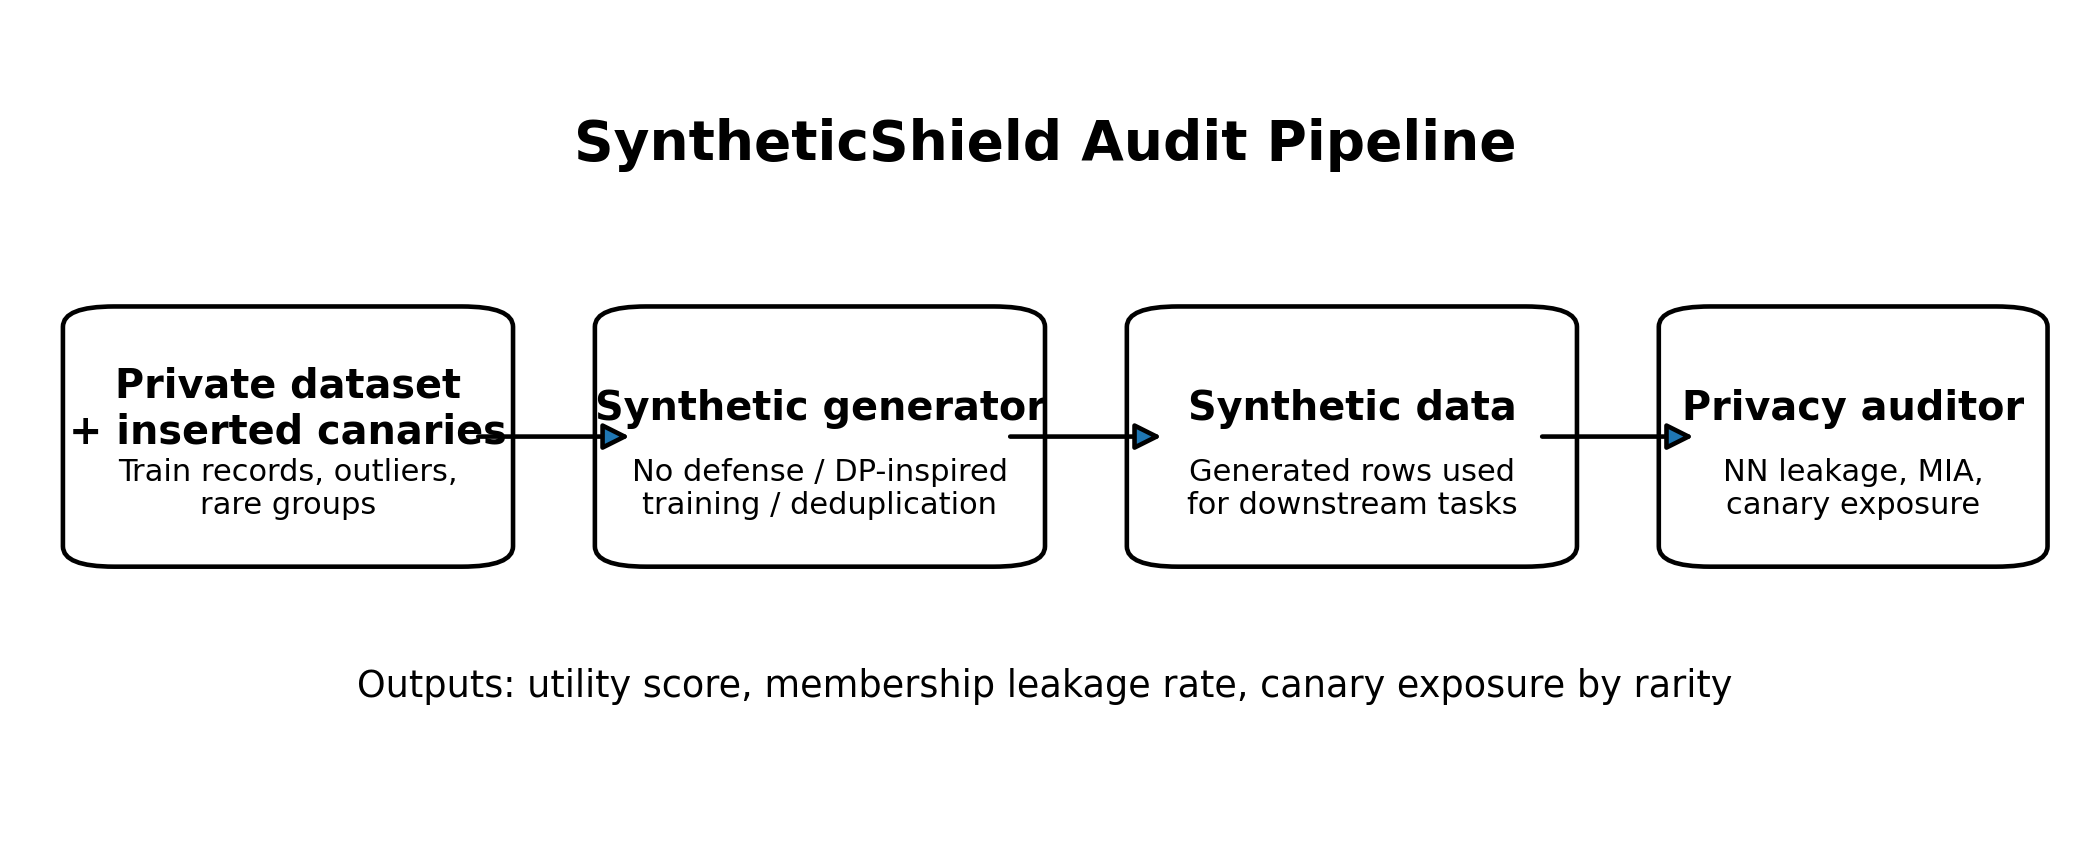
\includegraphics[width=0.95\textwidth]{../outputs/figures/main.png}
    \caption{SyntheticShield audit pipeline. A private dataset with inserted canaries is used to train a synthetic data generator. The generated samples are then passed to a privacy auditor that measures utility, membership leakage, and canary exposure.}
    \label{fig:main}
\end{figure*}

\subsection{Canary insertion}
Canaries are synthetic private records inserted into the training data before generator fitting. Each canary is assigned a rarity strength that controls how far its feature vector is from the ordinary data manifold. A generator that memorizes private rows should emit samples close to these canaries, while a safer generator should model only aggregate structure and avoid reproducing rare records.

\subsection{Generators and defenses}
We compare three generator settings. The \emph{no-defense} setting uses a memorization-prone bootstrap generator that resamples private rows and adds small noise. The \emph{DP-training} setting uses clipped features and noise-added Gaussian parameters. This setting is DP-inspired but does not claim a formal privacy guarantee. The \emph{deduplication} setting removes duplicate and extreme outlier rows before fitting a stronger-noise bootstrap generator.

\subsection{Privacy metrics}
For each candidate record $x$, SyntheticShield computes a nearest-neighbor distance to the synthetic release $S$:
\begin{equation}
    d(x,S) = \min_{s \in S} \lVert x - s \rVert_2.
\end{equation}
Membership inference uses $-d(x,S)$ as the attack score. We report attack AUC and leakage rate at 5\% false-positive rate. Canary exposure is measured as the fraction of canaries whose nearest synthetic neighbor is within a fixed threshold.

\section{Experimental Setup}
The benchmark uses a binary tabular classification dataset with standardized continuous features. We split the base records into private training and held-out non-member test sets, insert rare canaries into the private split, and generate synthetic samples from each defense configuration. Utility is measured with train-on-synthetic-test-on-real (TSTR): a logistic regression classifier is trained on synthetic samples and evaluated on real held-out records. Each configuration is repeated across multiple random seeds.

\section{Results}
Figure~\ref{fig:results} shows the three primary result panels produced by the repository.

\begin{figure*}[t]
    \centering
    \begin{subfigure}[t]{0.32\textwidth}
        \centering
        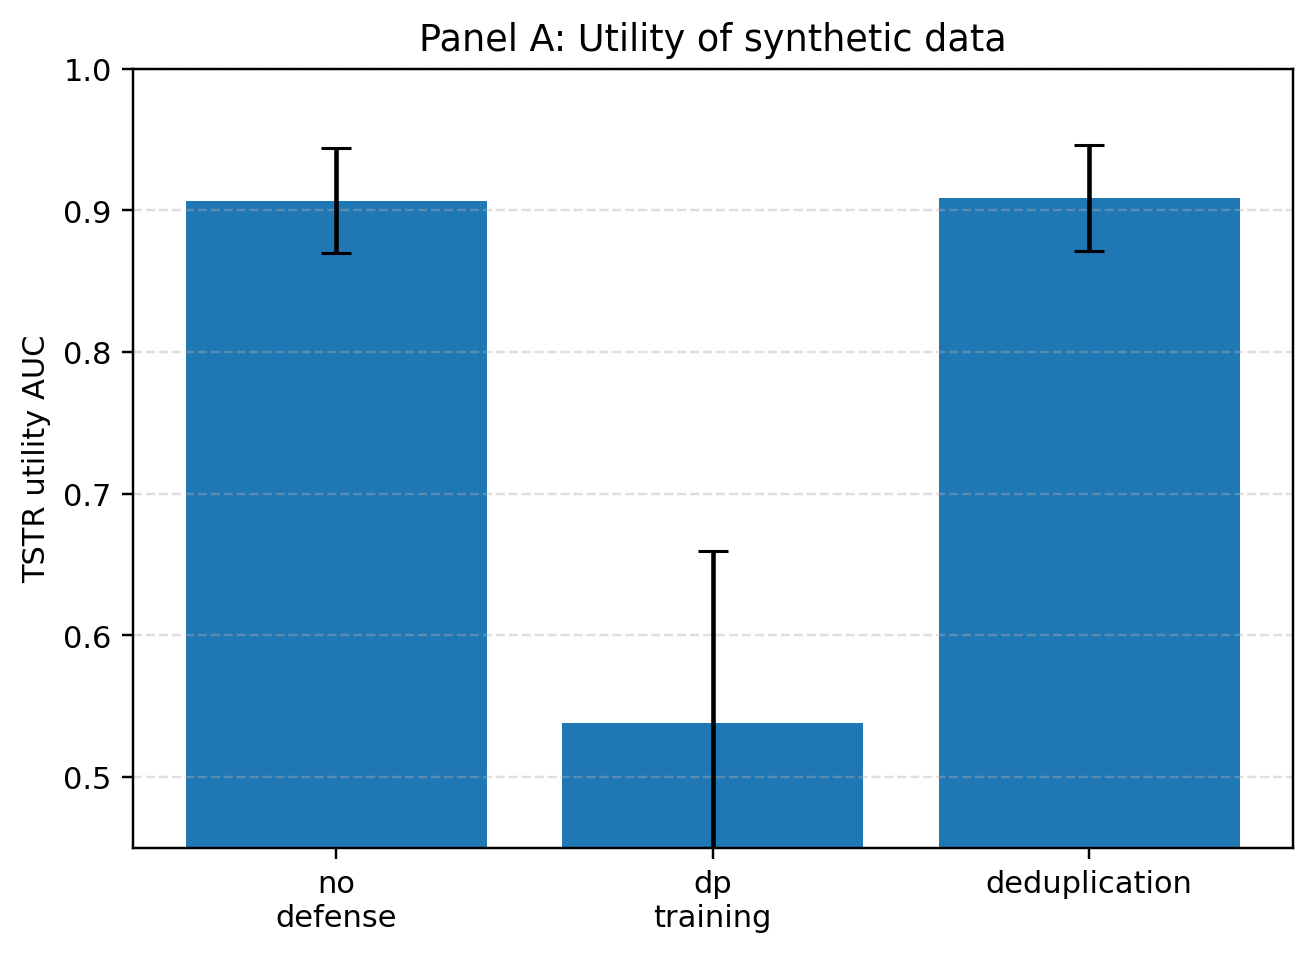
\includegraphics[width=\linewidth]{../outputs/figures/figure2.png}
        \caption{Utility of synthetic data.}
    \end{subfigure}
    \hfill
    \begin{subfigure}[t]{0.32\textwidth}
        \centering
        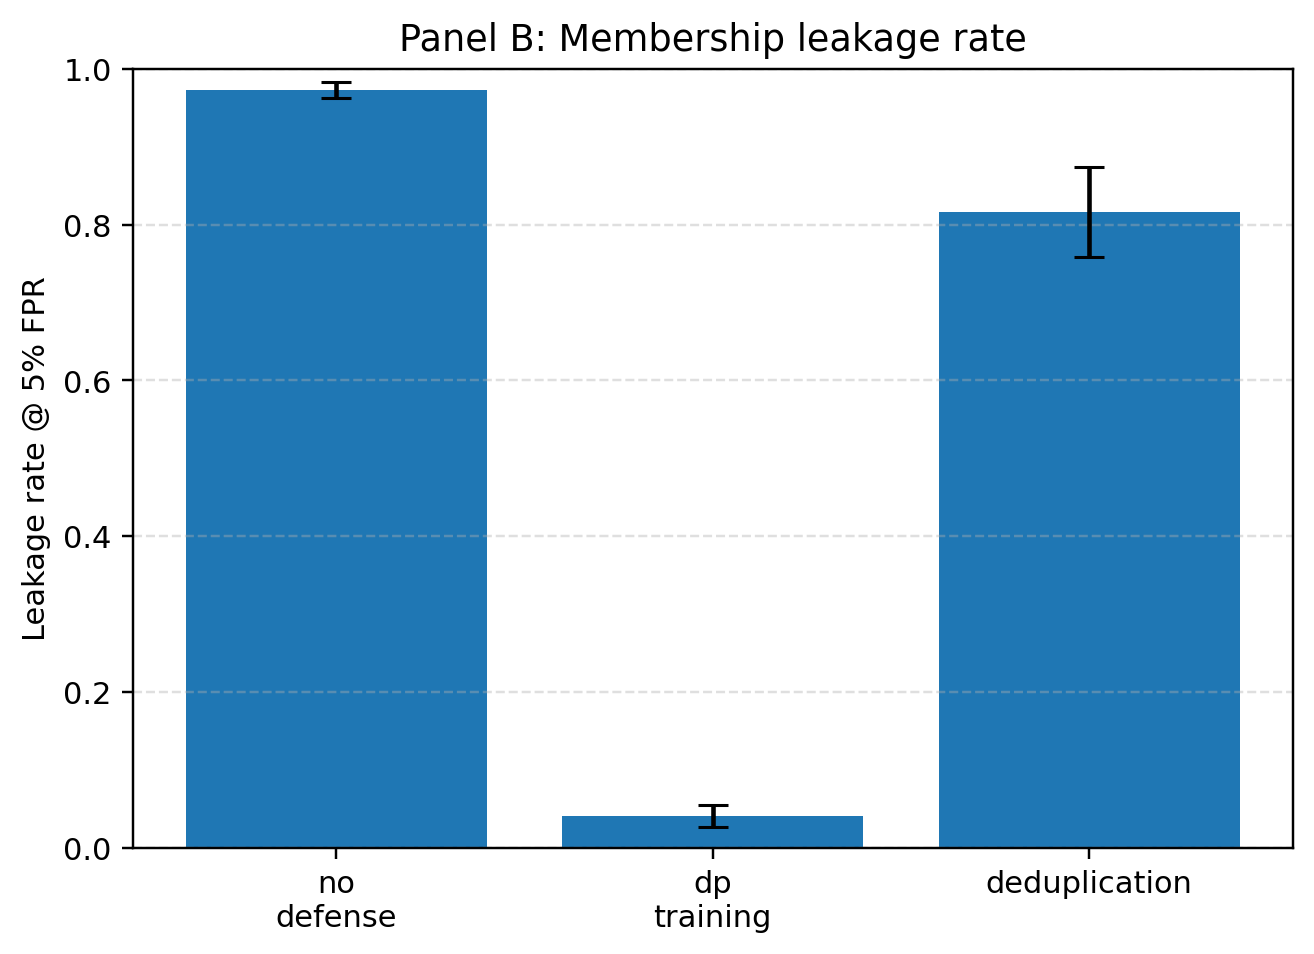
\includegraphics[width=\linewidth]{../outputs/figures/figure3.png}
        \caption{Membership leakage rate.}
    \end{subfigure}
    \hfill
    \begin{subfigure}[t]{0.32\textwidth}
        \centering
        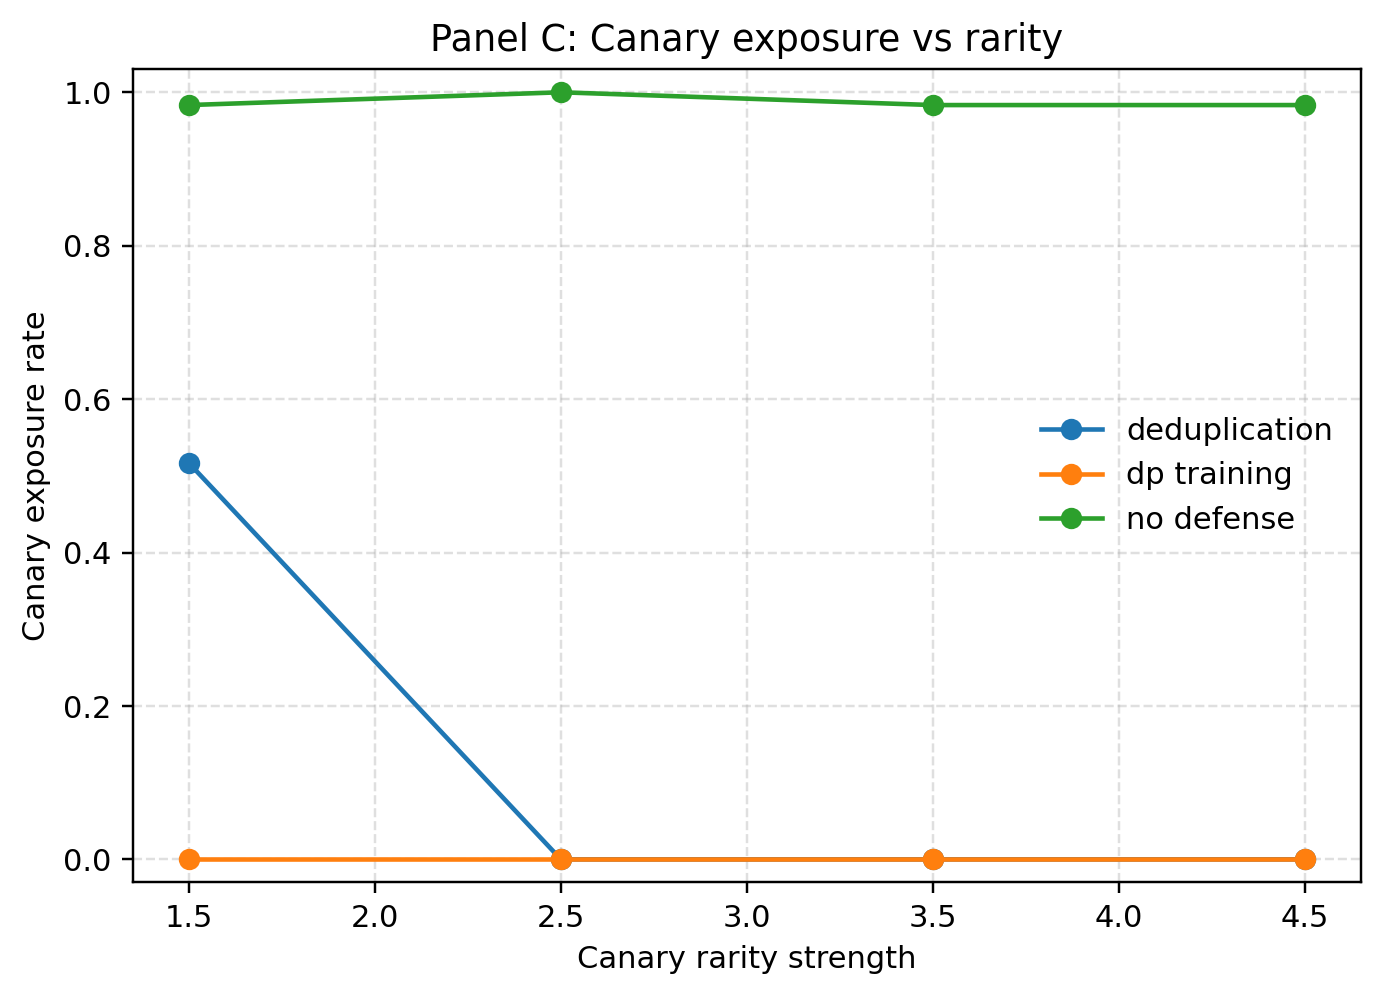
\includegraphics[width=\linewidth]{../outputs/figures/figure4.png}
        \caption{Canary exposure by rarity.}
    \end{subfigure}
    \caption{SyntheticShield result panels. The no-defense generator generally preserves utility but leaks more membership and canary information. DP-inspired training and deduplication reduce exposure, with a potential utility trade-off.}
    \label{fig:results}
\end{figure*}

The no-defense generator is expected to obtain strong utility because it resamples from the private distribution. However, this behavior also creates privacy risk: private records and canaries can appear very close to generated samples. The DP-inspired generator reduces direct copying by sampling from noisy aggregate parameters, while deduplication removes rare or repeated records before generation. These results demonstrate why synthetic data should be audited rather than assumed safe.

\section{Discussion}
SyntheticShield is intentionally simple and transparent. Its goal is not to provide a final privacy proof, but to expose generator behavior that should trigger deeper review before data release. The audit can be extended to mixed categorical data, text embeddings, stronger generative models, and formal DP generators. Future versions can also support attribute inference, subgroup leakage, and report generation for model cards or data cards.

\section{Limitations}
The current implementation uses a controlled tabular benchmark and simple generators. The DP-inspired defense is not a certified differentially private mechanism. Results should therefore be interpreted as an audit demonstration rather than a deployment-ready privacy guarantee. Real deployments should combine empirical auditing with formal privacy analysis, domain-specific risk thresholds, and governance review.

\section{Code Availability}
The SyntheticShield codebase is organized as a reproducible research repository with scripts, configuration files, generated result tables, and paper figures. The repository can be run with the commands in the README to regenerate all experiment outputs.

\section{Conclusion}
This paper presented \textsc{SyntheticShield}, a practical framework for measuring privacy leakage in synthetic data. By combining canary insertion, nearest-neighbor auditing, membership inference, and utility evaluation, SyntheticShield helps identify when synthetic data generators memorize rare private records. The results support a central message: synthetic data releases require privacy audits, especially when rare or outlier records may be present in the training set.

\bibliographystyle{plain}
\bibliography{references}

\end{document}
